\section{Extension Framework使用到的v8 API}

FunctionTemplate类是Function类的模板类,可以理解为设置Function的公共特性,
通过FunctionTemplate类new出来的Function类就拥有这些特性。相当于页面的function。
\begin{spacing}{1.0}
\begin{lstlisting}[language={C++}]
/**
@brief new一个FunctionTemplate对象

@param[in] isolate表示一个独立的v8引擎实例,每个实例维护不同的状态
@param[in] callback是回调函数,创建实例或方法被调用时会调用
@param[in] data表示给回调函数传递的额外的参数
@return 返回FunctionTemplate对象
*/
static Local<FunctionTemplate> New(
    Isolate* isolate, FunctionCallback callback = 0,
    Local<Value> data = Local<Value>(),
    Local<Signature> signature = Local<Signature>(), int length = 0,
    ConstructorBehavior behavior = ConstructorBehavior::kAllow);

/**
 * Set the call-handler callback for a FunctionTemplate.  This
 * callback is called whenever the function created from this
 * FunctionTemplate is called.
 */
void SetCallHandler(FunctionCallback callback,
    Local<Value> data = Local<Value>());
\end{lstlisting}
\end{spacing}

ObjectTemplate类是Object类的模板类,可以理解为设置Object的公共特性,
通过ObjectTemplate类new出来的Object类就拥有这些特性。相当于页面的object。
\begin{spacing}{1.0}
\begin{lstlisting}[language={C++}]
/**
@brief new一个ObjectTemplate对象

@param[in] isolate表示一个独立的v8引擎实例,每个实例维护不同的状态
@param[in] constructor是默认构造函数,只用于创建实例时会调用
@return 返回ObjectTemplate对象
*/
static Local<ObjectTemplate> New(
    Isolate* isolate,
    Local<FunctionTemplate> constructor = Local<FunctionTemplate>());

/**
@brief new一个Object对象实例

@param[in] context表示JavaScript代码运行环境上下文
@return 返回Object对象
*/
V8_WARN_UNUSED_RESULT MaybeLocal<Object> NewInstance(Local<Context> context);

/**
@brief 能够指定JavaScript访问对象属性时的一个callback

@param[in] getter表示获取属性时会被调用的callback
@param[in] setter表示设置属性时会被调用的callback
*/
void SetNamedPropertyHandler(NamedPropertyGetterCallback getter,
    NamedPropertySetterCallback setter = 0,
    NamedPropertyQueryCallback query = 0,
    NamedPropertyDeleterCallback deleter = 0,
    NamedPropertyEnumeratorCallback enumerator = 0,
    Local<Value> data = Local<Value>());
    
/**
@brief 通过这个模板生成的Object对象可以设置的内部field的数量

@param[in] value表示设置内部field的数量
*/
void SetInternalFieldCount(int value);
\end{lstlisting}
\end{spacing}

Object类是一个实例对象
\begin{spacing}{1.0}
\begin{lstlisting}[language={C++}]
/**
@brief 设置Object的内部field

@param[in] index表示Object的内部field的索引值,必须小于SetInternalFieldCount函数传入的值
@param[in] value表示Object的内部field值
*/
void SetInternalField(int index, Local<Value> value);
\end{lstlisting}
\end{spacing}

其他
\begin{spacing}{1.0}
\begin{lstlisting}[language={C++}]
/**
 * A map that uses Global as value and std::map as the backing
 * implementation. Globals are held non-weak.
 *
 * C++11 embedders don't need this class, as they can use
 * Global directly in std containers.
 */
template <typename K, typename V,
          typename Traits = DefaultGlobalMapTraits<K, V> >
class StdGlobalValueMap : public GlobalValueMap<K, V, Traits> {
 public:
  explicit StdGlobalValueMap(Isolate* isolate)
      : GlobalValueMap<K, V, Traits>(isolate) {}
};
\end{lstlisting}
\end{spacing}

\section{extension framework架构分析}
\begin{figure}[H] 
  \centering 
  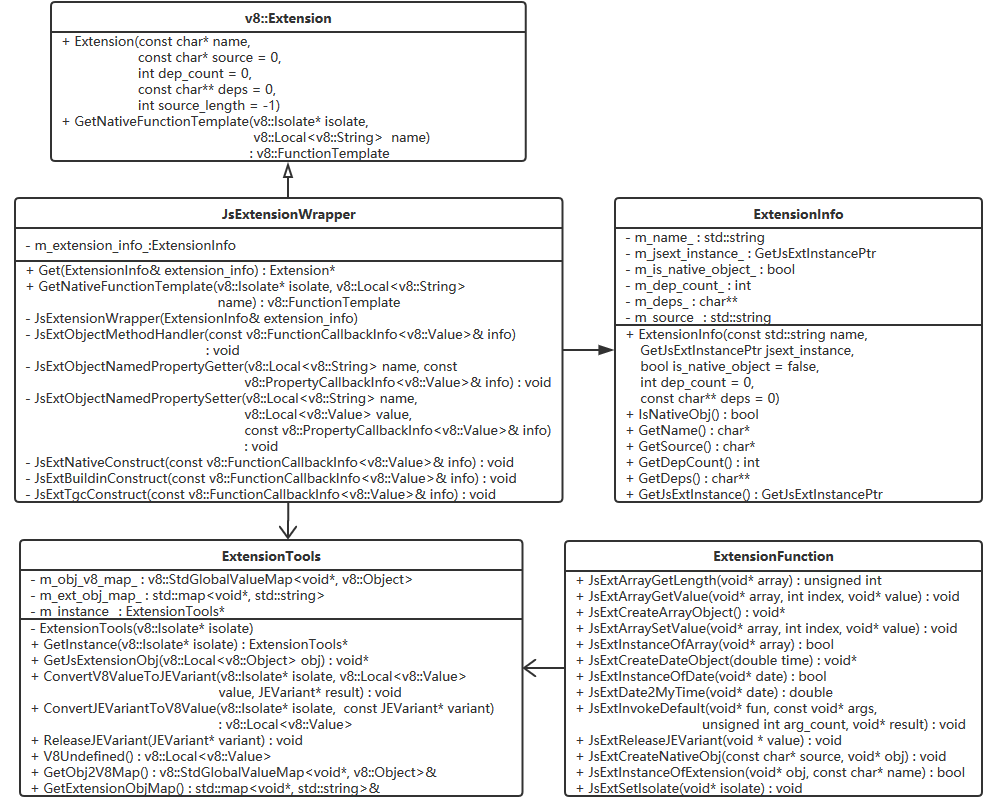
\includegraphics[width=\textwidth]{image/extension_framework/extension_framework_class.png} 
  \caption{extension framwork静态类图} \label{fig:extension_framework_class} 
\end{figure}

如第图~\ref{fig:extension_framework_class}所示:
v8扩展机制主要是继承v8内置的Extension类,通过重写其GetNativeFunctionTemplate方法来获取FunctionTemplate对象;
JsExtensionWrapper类主要就是封装创建出来的FunctionTemplate对象的一些特性,比如构造函数,属性拦截器,方法执行;
ExtensionInfo类主要记录了创建v8扩展所有需要的关键信息;ExtensionTools类主要是提供简易的函数,比如通过v8::Object类获取ExtensionBase对象,
将v8变量转换为扩展变量,将扩展变量转换为v8变量,释放扩展变量等;ExtensionFunction主要提供常用对外接口给js扩展调用。

\begin{figure}[H] 
  \centering 
  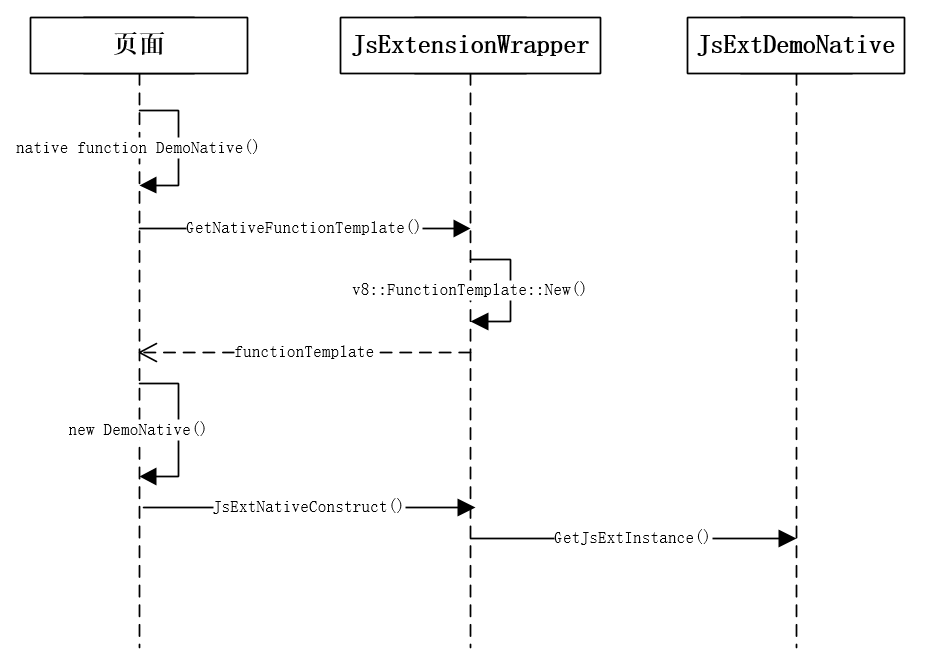
\includegraphics[width=\textwidth]{image/extension_framework/extension_construct_sequence.png} 
  \caption{js扩展对象创建时序图} \label{fig:extension_construct_sequence} 
\end{figure}

js扩展对象创建时序图如图~\ref{fig:extension_construct_sequence}所示:
\begin{itemize}
  \item 在页面加载时,v8::extension会注入页面代码native function DemoNative(),此时v8就会去创建DemoNative对应functionTemplate模板类。
  \item 当web开发人员在页面使用new DemoNative()时,functionTemplate模板类就会返回一个v8::Object实例对象给页面。
  \item 同理,针对内置对象,v8::extension会注入页面代码native function DemoBuildin()和var DemoBuildin = DemoBuildin()两段代码,
  此时由于DemoBuildin变量覆盖了DemoBuildin方法名,所以只能通过DemoBuildin执行对应方法和函数,不能再被new。
\end{itemize}

\begin{figure}[H] 
  \centering 
  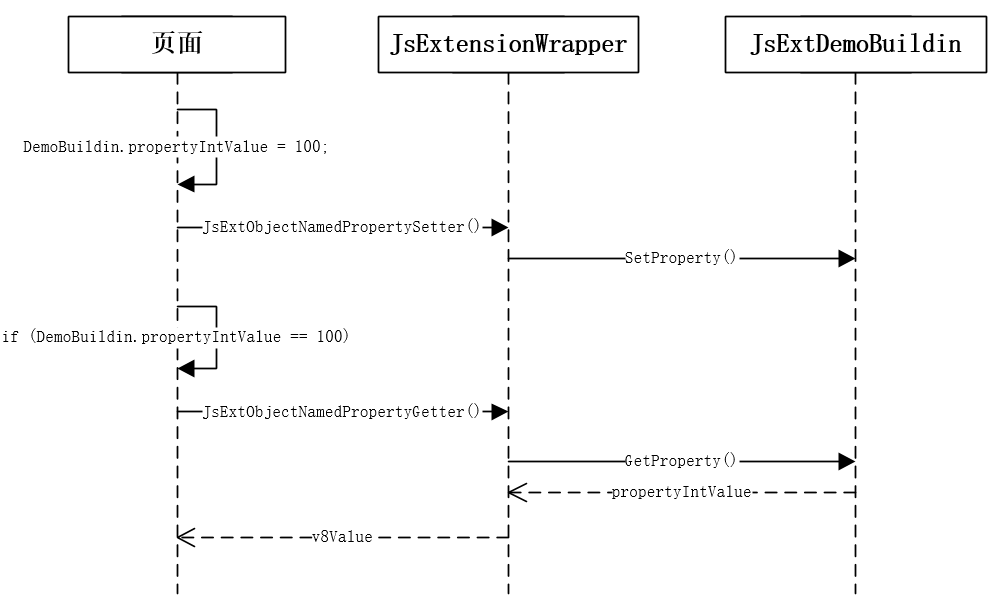
\includegraphics[width=\textwidth]{image/extension_framework/extension_property_sequence.png} 
  \caption{js扩展对象属性访问时序图} \label{fig:extension_property_sequence} 
\end{figure}

js扩展对象属性访问时序图如图~\ref{fig:extension_property_sequence}所示:
\begin{itemize}
  \item 由于在创建DemoBuildin对象时,对其ObjectTemplate模板类设置了拦截器特性,所以任何属性访问都会调用到拦截器的回调方法里。
\end{itemize}

\begin{figure}[H] 
  \centering 
  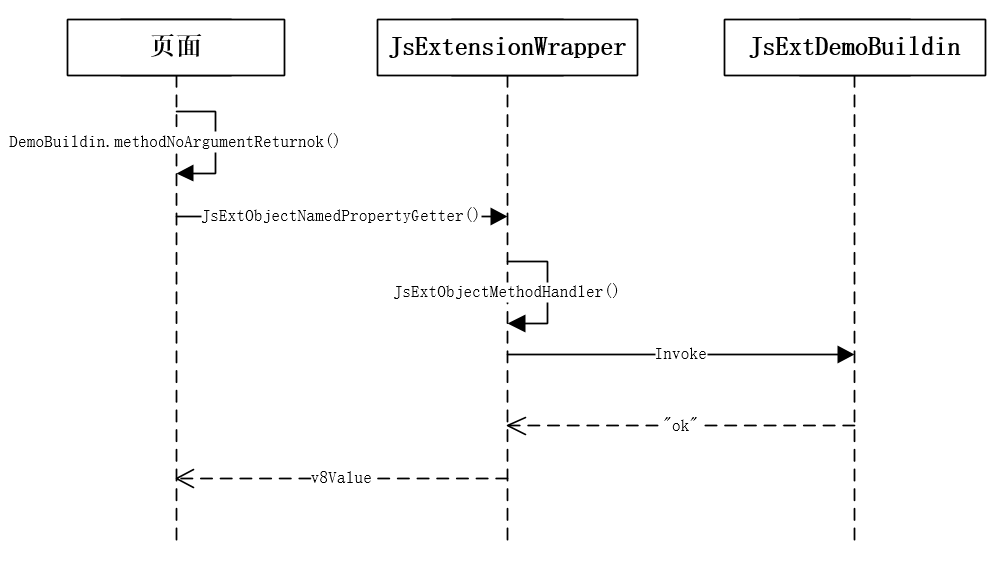
\includegraphics[width=\textwidth]{image/extension_framework/extension_function_sequence.png} 
  \caption{js扩展对象方法访问时序图} \label{fig:extension_function_sequence} 
\end{figure}

js扩展对象方法访问时序图如图~\ref{fig:extension_function_sequence}所示:
\begin{itemize}
  \item 同获取属性流程一致,当在拦截器回调函数里查询,如果属性没找到调用名,就去方法里找。
\end{itemize}

\section{Extension Framework垃圾回收机制}

对于内置对象,每次跳转页面,都会去调用其构造函数,此时回收机制的做法是先delete上个页面new出来的js扩展实例对象,再重新new一个js扩展实例对象,
然后绑定到v8 Object对象里。
\begin{spacing}{1.0}
\begin{lstlisting}[language={C++}]
void* delete_obj = ExtensionTools::GetJsExtensionObj(v8_obj);
  if (delete_obj) {
    ExtensionBase* ext_base = static_cast<ExtensionBase*>(delete_obj);
    delete ext_base;
    ext_base = NULL;
  }

  void* new_obj = NULL;
  extension_info->GetJsExtInstance()(NULL, 0, &new_obj);
  v8_obj->SetInternalField(ExtensionTools::JsExtBaseInternalField, v8::External::New(isolate, new_obj));
\end{lstlisting}
\end{spacing}

对于本地对象,每次创建对象时,我们会通过一个std::map保存js扩展实例对象指针以及name,当跳转页面,都会去调用tgc内置对象其构造函数,
将这个map里js扩展实例对象指针全部delete掉。
\begin{spacing}{1.0}
\begin{lstlisting}[language={C++}]
//在构造函数中将js扩展实例对象指针以及name保存到一个map中
void JsExtensionWrapper::JsExtNativeConstruct(const FunctionCallbackInfo<v8::Value>& info) {
  ...
  ExtensionTools* extension_tools = ExtensionTools::GetInstance(isolate);
  extension_tools->GetExtensionObjMap().insert(std::pair<void*, std::string>(new_obj, extension_info->GetName()));
  ...
}

//在tgc内置对象构造函数中将map中的js扩展实例对象指针全部delete掉
void JsExtensionWrapper::JsExtTgcConstruct(const FunctionCallbackInfo<v8::Value>& info) {
  ...
  ExtensionTools* extension_tools = ExtensionTools::GetInstance(isolate);
  std::map<void*, std::string>::iterator it;
  for (it = extension_tools->GetExtensionObjMap().begin(); it != extension_tools->GetExtensionObjMap().end(); it++) {
    ExtensionBase* ext_base = static_cast<ExtensionBase*>(it->first);
    if (ext_base) {
      delete ext_base;
      ext_base = NULL;
    }
  }
  ...
}
\end{lstlisting}
\end{spacing}



%---------------------------------------------------------------------

\ifx\withtbrowser\undefined
\else
\section{Extension Framework使用到的v8 API}

FunctionTemplate类是Function类的模板类,可以理解为设置Function的公共特性,
通过FunctionTemplate类new出来的Function类就拥有这些特性。相当于页面的function。
\begin{spacing}{1.0}
\begin{lstlisting}[language={C++}]
/**
@brief new一个FunctionTemplate对象

@param[in] isolate表示一个独立的v8引擎实例,每个实例维护不同的状态
@param[in] callback是回调函数,创建实例或方法被调用时会调用
@param[in] data表示给回调函数传递的额外的参数
@return 返回FunctionTemplate对象
*/
static Local<FunctionTemplate> New(
    Isolate* isolate, FunctionCallback callback = 0,
    Local<Value> data = Local<Value>(),
    Local<Signature> signature = Local<Signature>(), int length = 0,
    ConstructorBehavior behavior = ConstructorBehavior::kAllow);

/**
 * Set the call-handler callback for a FunctionTemplate.  This
 * callback is called whenever the function created from this
 * FunctionTemplate is called.
 */
void SetCallHandler(FunctionCallback callback,
    Local<Value> data = Local<Value>());
\end{lstlisting}
\end{spacing}

ObjectTemplate类是Object类的模板类,可以理解为设置Object的公共特性,
通过ObjectTemplate类new出来的Object类就拥有这些特性。相当于页面的object。
\begin{spacing}{1.0}
\begin{lstlisting}[language={C++}]
/**
@brief new一个ObjectTemplate对象

@param[in] isolate表示一个独立的v8引擎实例,每个实例维护不同的状态
@param[in] constructor是默认构造函数,只用于创建实例时会调用
@return 返回ObjectTemplate对象
*/
static Local<ObjectTemplate> New(
    Isolate* isolate,
    Local<FunctionTemplate> constructor = Local<FunctionTemplate>());

/**
@brief new一个Object对象实例

@param[in] context表示JavaScript代码运行环境上下文
@return 返回Object对象
*/
V8_WARN_UNUSED_RESULT MaybeLocal<Object> NewInstance(Local<Context> context);

/**
@brief 能够指定JavaScript访问对象属性时的一个callback

@param[in] getter表示获取属性时会被调用的callback
@param[in] setter表示设置属性时会被调用的callback
*/
void SetNamedPropertyHandler(NamedPropertyGetterCallback getter,
    NamedPropertySetterCallback setter = 0,
    NamedPropertyQueryCallback query = 0,
    NamedPropertyDeleterCallback deleter = 0,
    NamedPropertyEnumeratorCallback enumerator = 0,
    Local<Value> data = Local<Value>());
    
/**
@brief 通过这个模板生成的Object对象可以设置的内部field的数量

@param[in] value表示设置内部field的数量
*/
void SetInternalFieldCount(int value);
\end{lstlisting}
\end{spacing}

Object类是一个实例对象
\begin{spacing}{1.0}
\begin{lstlisting}[language={C++}]
/**
@brief 设置Object的内部field

@param[in] index表示Object的内部field的索引值,必须小于SetInternalFieldCount函数传入的值
@param[in] value表示Object的内部field值
*/
void SetInternalField(int index, Local<Value> value);
\end{lstlisting}
\end{spacing}

其他
\begin{spacing}{1.0}
\begin{lstlisting}[language={C++}]
/**
 * A map that uses Global as value and std::map as the backing
 * implementation. Globals are held non-weak.
 *
 * C++11 embedders don't need this class, as they can use
 * Global directly in std containers.
 */
template <typename K, typename V,
          typename Traits = DefaultGlobalMapTraits<K, V> >
class StdGlobalValueMap : public GlobalValueMap<K, V, Traits> {
 public:
  explicit StdGlobalValueMap(Isolate* isolate)
      : GlobalValueMap<K, V, Traits>(isolate) {}
};
\end{lstlisting}
\end{spacing}

\section{extension framework架构分析}
\begin{figure}[H] 
  \centering 
  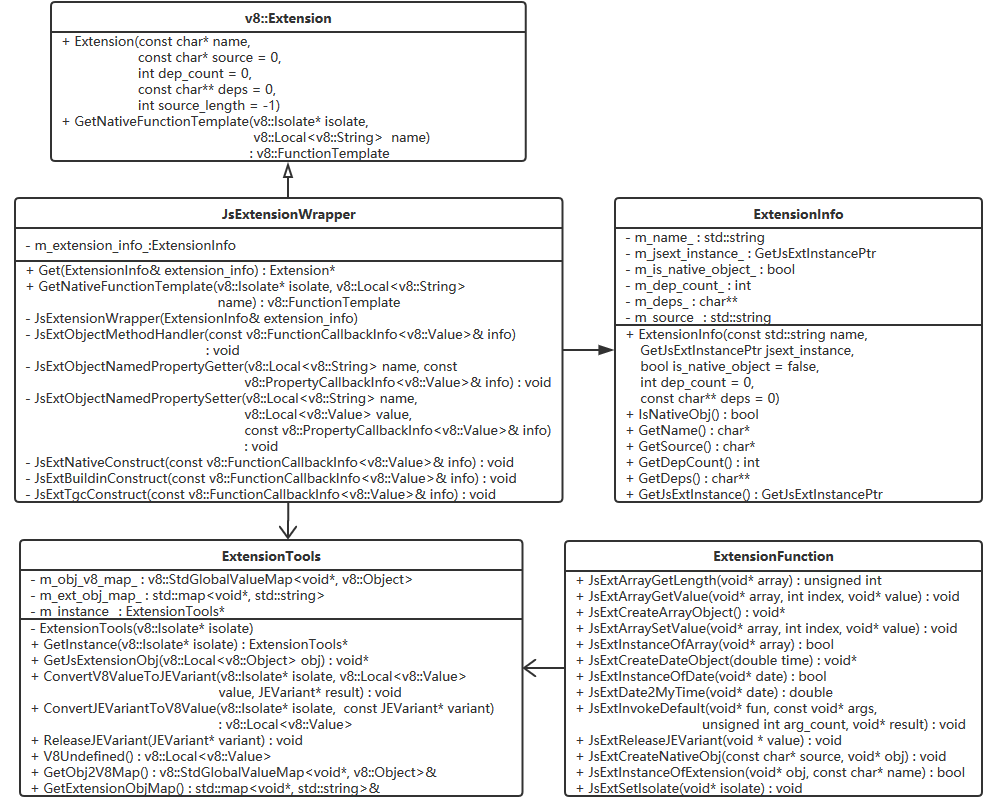
\includegraphics[width=\textwidth]{image/extension_framework/extension_framework_class.png} 
  \caption{extension framwork静态类图} \label{fig:extension_framework_class} 
\end{figure}

如第图~\ref{fig:extension_framework_class}所示:
v8扩展机制主要是继承v8内置的Extension类,通过重写其GetNativeFunctionTemplate方法来获取FunctionTemplate对象;
JsExtensionWrapper类主要就是封装创建出来的FunctionTemplate对象的一些特性,比如构造函数,属性拦截器,方法执行;
ExtensionInfo类主要记录了创建v8扩展所有需要的关键信息;ExtensionTools类主要是提供简易的函数,比如通过v8::Object类获取ExtensionBase对象,
将v8变量转换为扩展变量,将扩展变量转换为v8变量,释放扩展变量等;ExtensionFunction主要提供常用对外接口给js扩展调用。

\begin{figure}[H] 
  \centering 
  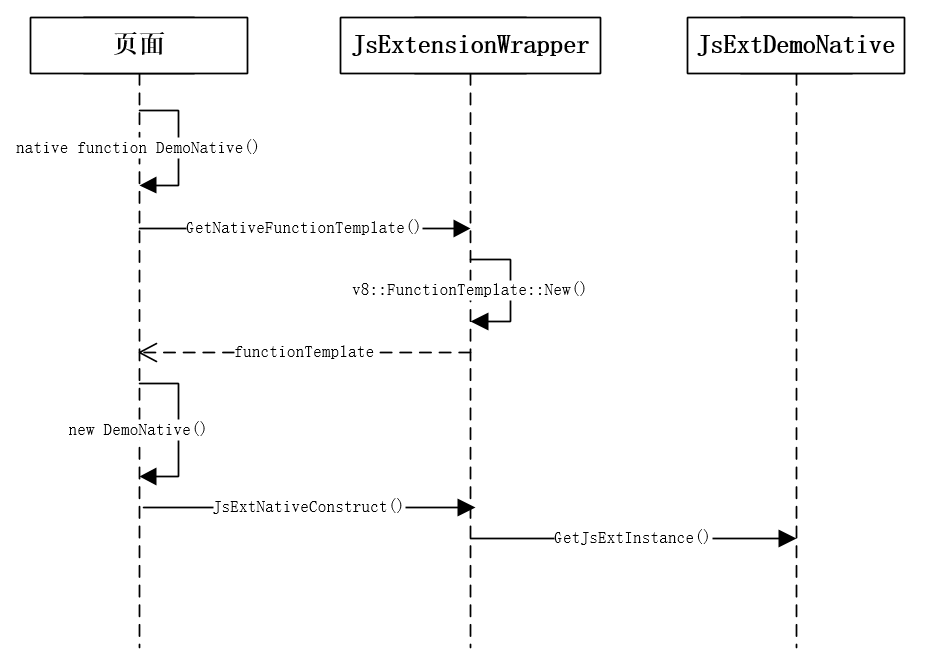
\includegraphics[width=\textwidth]{image/extension_framework/extension_construct_sequence.png} 
  \caption{js扩展对象创建时序图} \label{fig:extension_construct_sequence} 
\end{figure}

js扩展对象创建时序图如图~\ref{fig:extension_construct_sequence}所示:
\begin{itemize}
  \item 在页面加载时,v8::extension会注入页面代码native function DemoNative(),此时v8就会去创建DemoNative对应functionTemplate模板类。
  \item 当web开发人员在页面使用new DemoNative()时,functionTemplate模板类就会返回一个v8::Object实例对象给页面。
  \item 同理,针对内置对象,v8::extension会注入页面代码native function DemoBuildin()和var DemoBuildin = DemoBuildin()两段代码,
  此时由于DemoBuildin变量覆盖了DemoBuildin方法名,所以只能通过DemoBuildin执行对应方法和函数,不能再被new。
\end{itemize}

\begin{figure}[H] 
  \centering 
  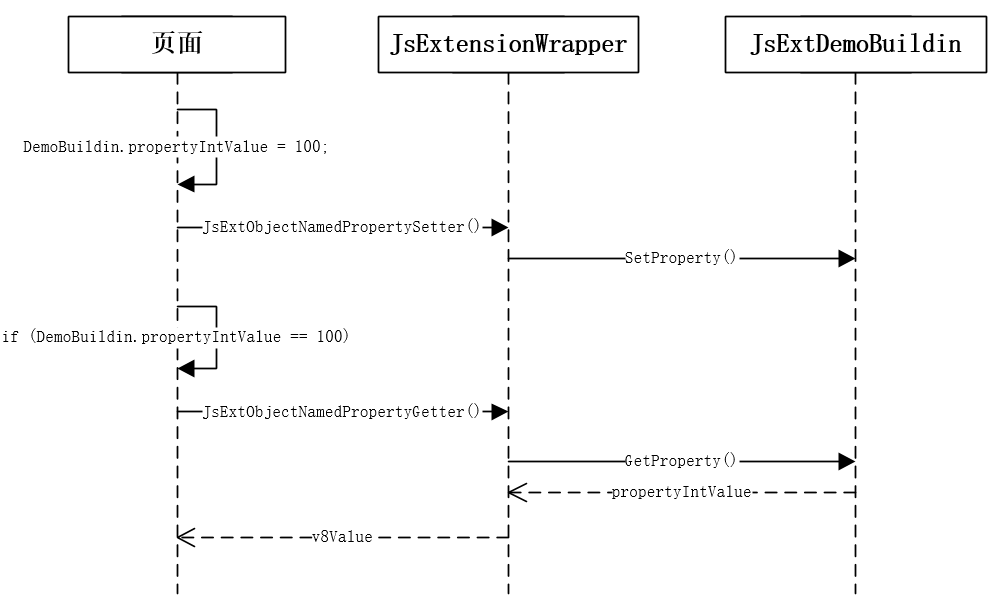
\includegraphics[width=\textwidth]{image/extension_framework/extension_property_sequence.png} 
  \caption{js扩展对象属性访问时序图} \label{fig:extension_property_sequence} 
\end{figure}

js扩展对象属性访问时序图如图~\ref{fig:extension_property_sequence}所示:
\begin{itemize}
  \item 由于在创建DemoBuildin对象时,对其ObjectTemplate模板类设置了拦截器特性,所以任何属性访问都会调用到拦截器的回调方法里。
\end{itemize}

\begin{figure}[H] 
  \centering 
  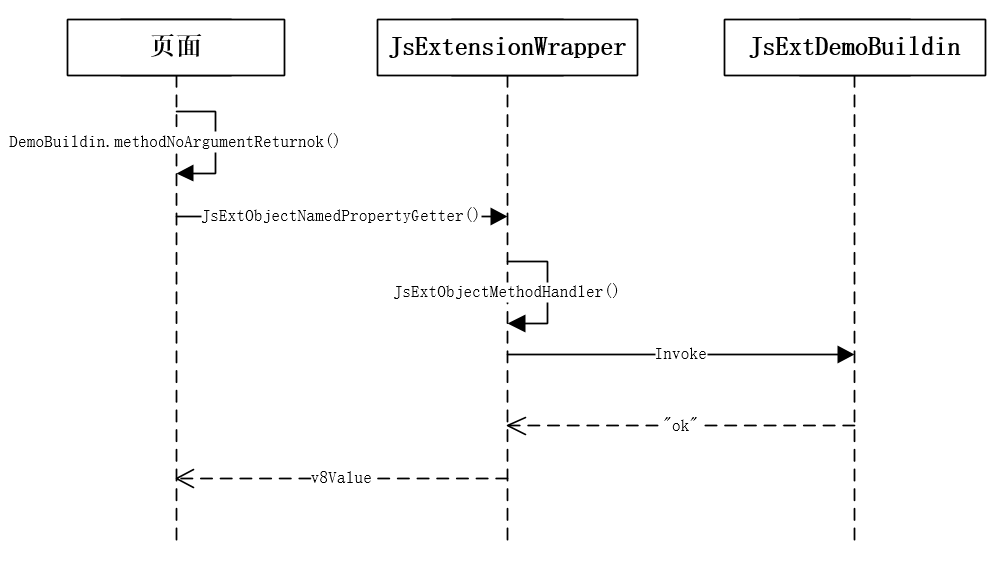
\includegraphics[width=\textwidth]{image/extension_framework/extension_function_sequence.png} 
  \caption{js扩展对象方法访问时序图} \label{fig:extension_function_sequence} 
\end{figure}

js扩展对象方法访问时序图如图~\ref{fig:extension_function_sequence}所示:
\begin{itemize}
  \item 同获取属性流程一致,当在拦截器回调函数里查询,如果属性没找到调用名,就去方法里找。
\end{itemize}

\section{Extension Framework垃圾回收机制}

对于内置对象,每次跳转页面,都会去调用其构造函数,此时回收机制的做法是先delete上个页面new出来的js扩展实例对象,再重新new一个js扩展实例对象,
然后绑定到v8 Object对象里。
\begin{spacing}{1.0}
\begin{lstlisting}[language={C++}]
void* delete_obj = ExtensionTools::GetJsExtensionObj(v8_obj);
  if (delete_obj) {
    ExtensionBase* ext_base = static_cast<ExtensionBase*>(delete_obj);
    delete ext_base;
    ext_base = NULL;
  }

  void* new_obj = NULL;
  extension_info->GetJsExtInstance()(NULL, 0, &new_obj);
  v8_obj->SetInternalField(ExtensionTools::JsExtBaseInternalField, v8::External::New(isolate, new_obj));
\end{lstlisting}
\end{spacing}

对于本地对象,每次创建对象时,我们会通过一个std::map保存js扩展实例对象指针以及name,当跳转页面,都会去调用tgc内置对象其构造函数,
将这个map里js扩展实例对象指针全部delete掉。
\begin{spacing}{1.0}
\begin{lstlisting}[language={C++}]
//在构造函数中将js扩展实例对象指针以及name保存到一个map中
void JsExtensionWrapper::JsExtNativeConstruct(const FunctionCallbackInfo<v8::Value>& info) {
  ...
  ExtensionTools* extension_tools = ExtensionTools::GetInstance(isolate);
  extension_tools->GetExtensionObjMap().insert(std::pair<void*, std::string>(new_obj, extension_info->GetName()));
  ...
}

//在tgc内置对象构造函数中将map中的js扩展实例对象指针全部delete掉
void JsExtensionWrapper::JsExtTgcConstruct(const FunctionCallbackInfo<v8::Value>& info) {
  ...
  ExtensionTools* extension_tools = ExtensionTools::GetInstance(isolate);
  std::map<void*, std::string>::iterator it;
  for (it = extension_tools->GetExtensionObjMap().begin(); it != extension_tools->GetExtensionObjMap().end(); it++) {
    ExtensionBase* ext_base = static_cast<ExtensionBase*>(it->first);
    if (ext_base) {
      delete ext_base;
      ext_base = NULL;
    }
  }
  ...
}
\end{lstlisting}
\end{spacing}



%---------------------------------------------------------------------

\ifx\withtbrowser\undefined
\else
\section{Extension Framework使用到的v8 API}

FunctionTemplate类是Function类的模板类,可以理解为设置Function的公共特性,
通过FunctionTemplate类new出来的Function类就拥有这些特性。相当于页面的function。
\begin{spacing}{1.0}
\begin{lstlisting}[language={C++}]
/**
@brief new一个FunctionTemplate对象

@param[in] isolate表示一个独立的v8引擎实例,每个实例维护不同的状态
@param[in] callback是回调函数,创建实例或方法被调用时会调用
@param[in] data表示给回调函数传递的额外的参数
@return 返回FunctionTemplate对象
*/
static Local<FunctionTemplate> New(
    Isolate* isolate, FunctionCallback callback = 0,
    Local<Value> data = Local<Value>(),
    Local<Signature> signature = Local<Signature>(), int length = 0,
    ConstructorBehavior behavior = ConstructorBehavior::kAllow);

/**
 * Set the call-handler callback for a FunctionTemplate.  This
 * callback is called whenever the function created from this
 * FunctionTemplate is called.
 */
void SetCallHandler(FunctionCallback callback,
    Local<Value> data = Local<Value>());
\end{lstlisting}
\end{spacing}

ObjectTemplate类是Object类的模板类,可以理解为设置Object的公共特性,
通过ObjectTemplate类new出来的Object类就拥有这些特性。相当于页面的object。
\begin{spacing}{1.0}
\begin{lstlisting}[language={C++}]
/**
@brief new一个ObjectTemplate对象

@param[in] isolate表示一个独立的v8引擎实例,每个实例维护不同的状态
@param[in] constructor是默认构造函数,只用于创建实例时会调用
@return 返回ObjectTemplate对象
*/
static Local<ObjectTemplate> New(
    Isolate* isolate,
    Local<FunctionTemplate> constructor = Local<FunctionTemplate>());

/**
@brief new一个Object对象实例

@param[in] context表示JavaScript代码运行环境上下文
@return 返回Object对象
*/
V8_WARN_UNUSED_RESULT MaybeLocal<Object> NewInstance(Local<Context> context);

/**
@brief 能够指定JavaScript访问对象属性时的一个callback

@param[in] getter表示获取属性时会被调用的callback
@param[in] setter表示设置属性时会被调用的callback
*/
void SetNamedPropertyHandler(NamedPropertyGetterCallback getter,
    NamedPropertySetterCallback setter = 0,
    NamedPropertyQueryCallback query = 0,
    NamedPropertyDeleterCallback deleter = 0,
    NamedPropertyEnumeratorCallback enumerator = 0,
    Local<Value> data = Local<Value>());
    
/**
@brief 通过这个模板生成的Object对象可以设置的内部field的数量

@param[in] value表示设置内部field的数量
*/
void SetInternalFieldCount(int value);
\end{lstlisting}
\end{spacing}

Object类是一个实例对象
\begin{spacing}{1.0}
\begin{lstlisting}[language={C++}]
/**
@brief 设置Object的内部field

@param[in] index表示Object的内部field的索引值,必须小于SetInternalFieldCount函数传入的值
@param[in] value表示Object的内部field值
*/
void SetInternalField(int index, Local<Value> value);
\end{lstlisting}
\end{spacing}

其他
\begin{spacing}{1.0}
\begin{lstlisting}[language={C++}]
/**
 * A map that uses Global as value and std::map as the backing
 * implementation. Globals are held non-weak.
 *
 * C++11 embedders don't need this class, as they can use
 * Global directly in std containers.
 */
template <typename K, typename V,
          typename Traits = DefaultGlobalMapTraits<K, V> >
class StdGlobalValueMap : public GlobalValueMap<K, V, Traits> {
 public:
  explicit StdGlobalValueMap(Isolate* isolate)
      : GlobalValueMap<K, V, Traits>(isolate) {}
};
\end{lstlisting}
\end{spacing}

\section{extension framework架构分析}
\begin{figure}[H] 
  \centering 
  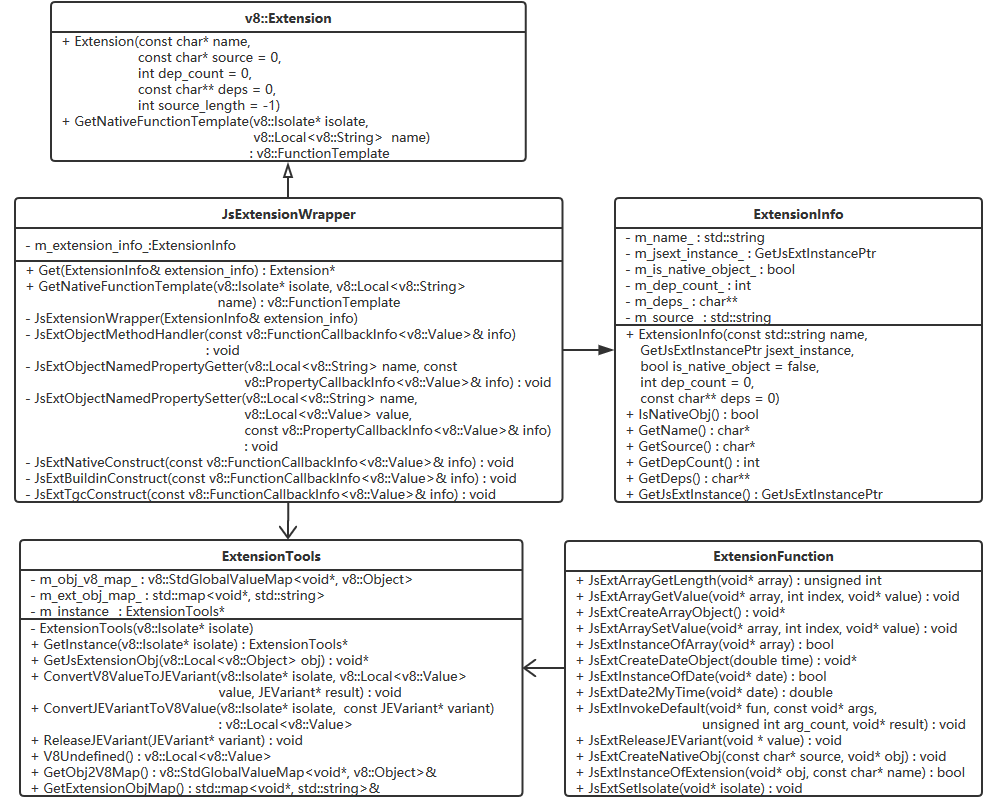
\includegraphics[width=\textwidth]{image/extension_framework/extension_framework_class.png} 
  \caption{extension framwork静态类图} \label{fig:extension_framework_class} 
\end{figure}

如第图~\ref{fig:extension_framework_class}所示:
v8扩展机制主要是继承v8内置的Extension类,通过重写其GetNativeFunctionTemplate方法来获取FunctionTemplate对象;
JsExtensionWrapper类主要就是封装创建出来的FunctionTemplate对象的一些特性,比如构造函数,属性拦截器,方法执行;
ExtensionInfo类主要记录了创建v8扩展所有需要的关键信息;ExtensionTools类主要是提供简易的函数,比如通过v8::Object类获取ExtensionBase对象,
将v8变量转换为扩展变量,将扩展变量转换为v8变量,释放扩展变量等;ExtensionFunction主要提供常用对外接口给js扩展调用。

\begin{figure}[H] 
  \centering 
  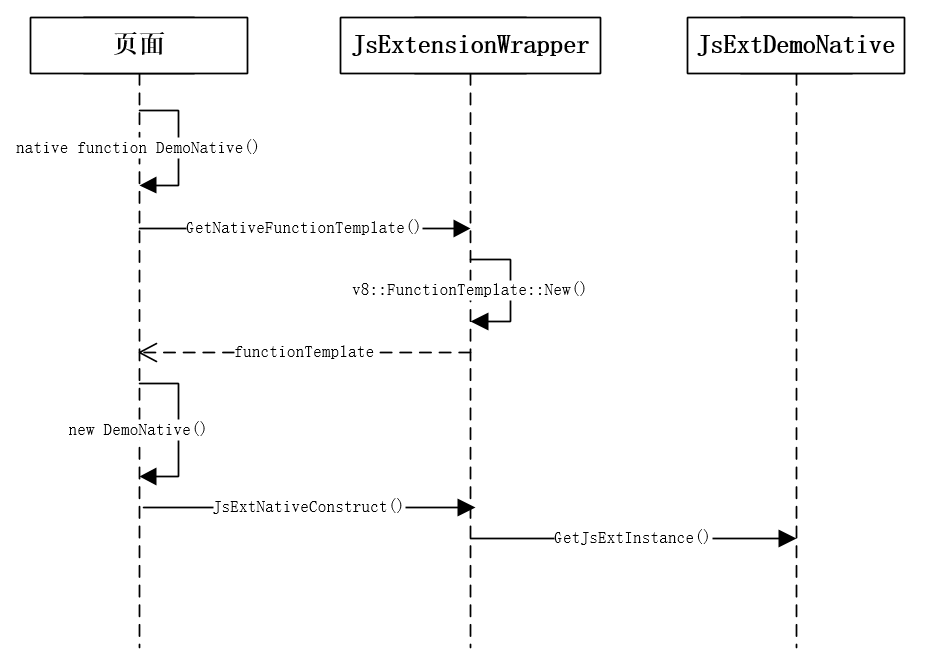
\includegraphics[width=\textwidth]{image/extension_framework/extension_construct_sequence.png} 
  \caption{js扩展对象创建时序图} \label{fig:extension_construct_sequence} 
\end{figure}

js扩展对象创建时序图如图~\ref{fig:extension_construct_sequence}所示:
\begin{itemize}
  \item 在页面加载时,v8::extension会注入页面代码native function DemoNative(),此时v8就会去创建DemoNative对应functionTemplate模板类。
  \item 当web开发人员在页面使用new DemoNative()时,functionTemplate模板类就会返回一个v8::Object实例对象给页面。
  \item 同理,针对内置对象,v8::extension会注入页面代码native function DemoBuildin()和var DemoBuildin = DemoBuildin()两段代码,
  此时由于DemoBuildin变量覆盖了DemoBuildin方法名,所以只能通过DemoBuildin执行对应方法和函数,不能再被new。
\end{itemize}

\begin{figure}[H] 
  \centering 
  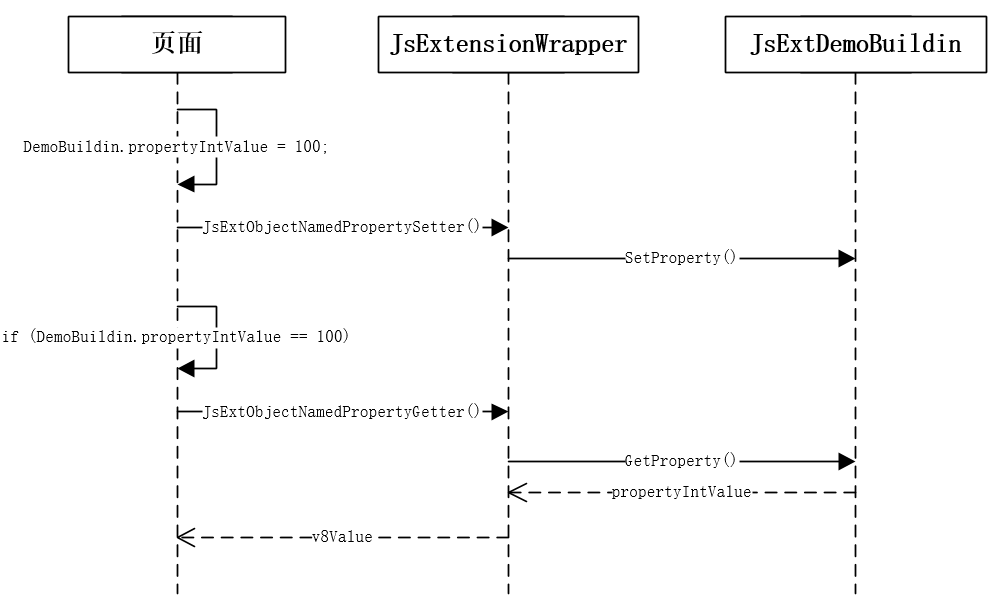
\includegraphics[width=\textwidth]{image/extension_framework/extension_property_sequence.png} 
  \caption{js扩展对象属性访问时序图} \label{fig:extension_property_sequence} 
\end{figure}

js扩展对象属性访问时序图如图~\ref{fig:extension_property_sequence}所示:
\begin{itemize}
  \item 由于在创建DemoBuildin对象时,对其ObjectTemplate模板类设置了拦截器特性,所以任何属性访问都会调用到拦截器的回调方法里。
\end{itemize}

\begin{figure}[H] 
  \centering 
  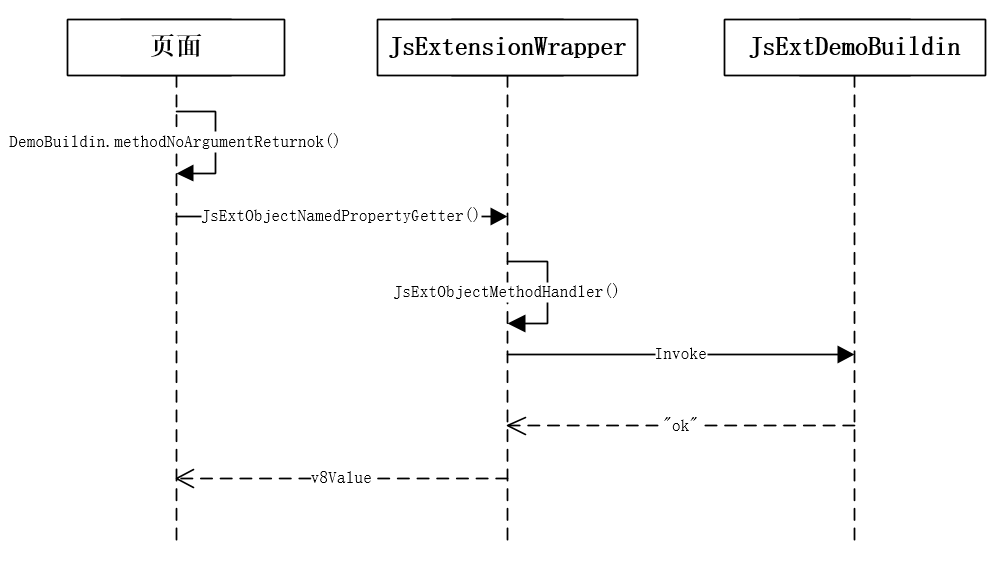
\includegraphics[width=\textwidth]{image/extension_framework/extension_function_sequence.png} 
  \caption{js扩展对象方法访问时序图} \label{fig:extension_function_sequence} 
\end{figure}

js扩展对象方法访问时序图如图~\ref{fig:extension_function_sequence}所示:
\begin{itemize}
  \item 同获取属性流程一致,当在拦截器回调函数里查询,如果属性没找到调用名,就去方法里找。
\end{itemize}

\section{Extension Framework垃圾回收机制}

对于内置对象,每次跳转页面,都会去调用其构造函数,此时回收机制的做法是先delete上个页面new出来的js扩展实例对象,再重新new一个js扩展实例对象,
然后绑定到v8 Object对象里。
\begin{spacing}{1.0}
\begin{lstlisting}[language={C++}]
void* delete_obj = ExtensionTools::GetJsExtensionObj(v8_obj);
  if (delete_obj) {
    ExtensionBase* ext_base = static_cast<ExtensionBase*>(delete_obj);
    delete ext_base;
    ext_base = NULL;
  }

  void* new_obj = NULL;
  extension_info->GetJsExtInstance()(NULL, 0, &new_obj);
  v8_obj->SetInternalField(ExtensionTools::JsExtBaseInternalField, v8::External::New(isolate, new_obj));
\end{lstlisting}
\end{spacing}

对于本地对象,每次创建对象时,我们会通过一个std::map保存js扩展实例对象指针以及name,当跳转页面,都会去调用tgc内置对象其构造函数,
将这个map里js扩展实例对象指针全部delete掉。
\begin{spacing}{1.0}
\begin{lstlisting}[language={C++}]
//在构造函数中将js扩展实例对象指针以及name保存到一个map中
void JsExtensionWrapper::JsExtNativeConstruct(const FunctionCallbackInfo<v8::Value>& info) {
  ...
  ExtensionTools* extension_tools = ExtensionTools::GetInstance(isolate);
  extension_tools->GetExtensionObjMap().insert(std::pair<void*, std::string>(new_obj, extension_info->GetName()));
  ...
}

//在tgc内置对象构造函数中将map中的js扩展实例对象指针全部delete掉
void JsExtensionWrapper::JsExtTgcConstruct(const FunctionCallbackInfo<v8::Value>& info) {
  ...
  ExtensionTools* extension_tools = ExtensionTools::GetInstance(isolate);
  std::map<void*, std::string>::iterator it;
  for (it = extension_tools->GetExtensionObjMap().begin(); it != extension_tools->GetExtensionObjMap().end(); it++) {
    ExtensionBase* ext_base = static_cast<ExtensionBase*>(it->first);
    if (ext_base) {
      delete ext_base;
      ext_base = NULL;
    }
  }
  ...
}
\end{lstlisting}
\end{spacing}



%---------------------------------------------------------------------

\ifx\withtbrowser\undefined
\else
\section{Extension Framework使用到的v8 API}

FunctionTemplate类是Function类的模板类,可以理解为设置Function的公共特性,
通过FunctionTemplate类new出来的Function类就拥有这些特性。相当于页面的function。
\begin{spacing}{1.0}
\begin{lstlisting}[language={C++}]
/**
@brief new一个FunctionTemplate对象

@param[in] isolate表示一个独立的v8引擎实例,每个实例维护不同的状态
@param[in] callback是回调函数,创建实例或方法被调用时会调用
@param[in] data表示给回调函数传递的额外的参数
@return 返回FunctionTemplate对象
*/
static Local<FunctionTemplate> New(
    Isolate* isolate, FunctionCallback callback = 0,
    Local<Value> data = Local<Value>(),
    Local<Signature> signature = Local<Signature>(), int length = 0,
    ConstructorBehavior behavior = ConstructorBehavior::kAllow);

/**
 * Set the call-handler callback for a FunctionTemplate.  This
 * callback is called whenever the function created from this
 * FunctionTemplate is called.
 */
void SetCallHandler(FunctionCallback callback,
    Local<Value> data = Local<Value>());
\end{lstlisting}
\end{spacing}

ObjectTemplate类是Object类的模板类,可以理解为设置Object的公共特性,
通过ObjectTemplate类new出来的Object类就拥有这些特性。相当于页面的object。
\begin{spacing}{1.0}
\begin{lstlisting}[language={C++}]
/**
@brief new一个ObjectTemplate对象

@param[in] isolate表示一个独立的v8引擎实例,每个实例维护不同的状态
@param[in] constructor是默认构造函数,只用于创建实例时会调用
@return 返回ObjectTemplate对象
*/
static Local<ObjectTemplate> New(
    Isolate* isolate,
    Local<FunctionTemplate> constructor = Local<FunctionTemplate>());

/**
@brief new一个Object对象实例

@param[in] context表示JavaScript代码运行环境上下文
@return 返回Object对象
*/
V8_WARN_UNUSED_RESULT MaybeLocal<Object> NewInstance(Local<Context> context);

/**
@brief 能够指定JavaScript访问对象属性时的一个callback

@param[in] getter表示获取属性时会被调用的callback
@param[in] setter表示设置属性时会被调用的callback
*/
void SetNamedPropertyHandler(NamedPropertyGetterCallback getter,
    NamedPropertySetterCallback setter = 0,
    NamedPropertyQueryCallback query = 0,
    NamedPropertyDeleterCallback deleter = 0,
    NamedPropertyEnumeratorCallback enumerator = 0,
    Local<Value> data = Local<Value>());
    
/**
@brief 通过这个模板生成的Object对象可以设置的内部field的数量

@param[in] value表示设置内部field的数量
*/
void SetInternalFieldCount(int value);
\end{lstlisting}
\end{spacing}

Object类是一个实例对象
\begin{spacing}{1.0}
\begin{lstlisting}[language={C++}]
/**
@brief 设置Object的内部field

@param[in] index表示Object的内部field的索引值,必须小于SetInternalFieldCount函数传入的值
@param[in] value表示Object的内部field值
*/
void SetInternalField(int index, Local<Value> value);
\end{lstlisting}
\end{spacing}

其他
\begin{spacing}{1.0}
\begin{lstlisting}[language={C++}]
/**
 * A map that uses Global as value and std::map as the backing
 * implementation. Globals are held non-weak.
 *
 * C++11 embedders don't need this class, as they can use
 * Global directly in std containers.
 */
template <typename K, typename V,
          typename Traits = DefaultGlobalMapTraits<K, V> >
class StdGlobalValueMap : public GlobalValueMap<K, V, Traits> {
 public:
  explicit StdGlobalValueMap(Isolate* isolate)
      : GlobalValueMap<K, V, Traits>(isolate) {}
};
\end{lstlisting}
\end{spacing}

\section{extension framework架构分析}
\begin{figure}[H] 
  \centering 
  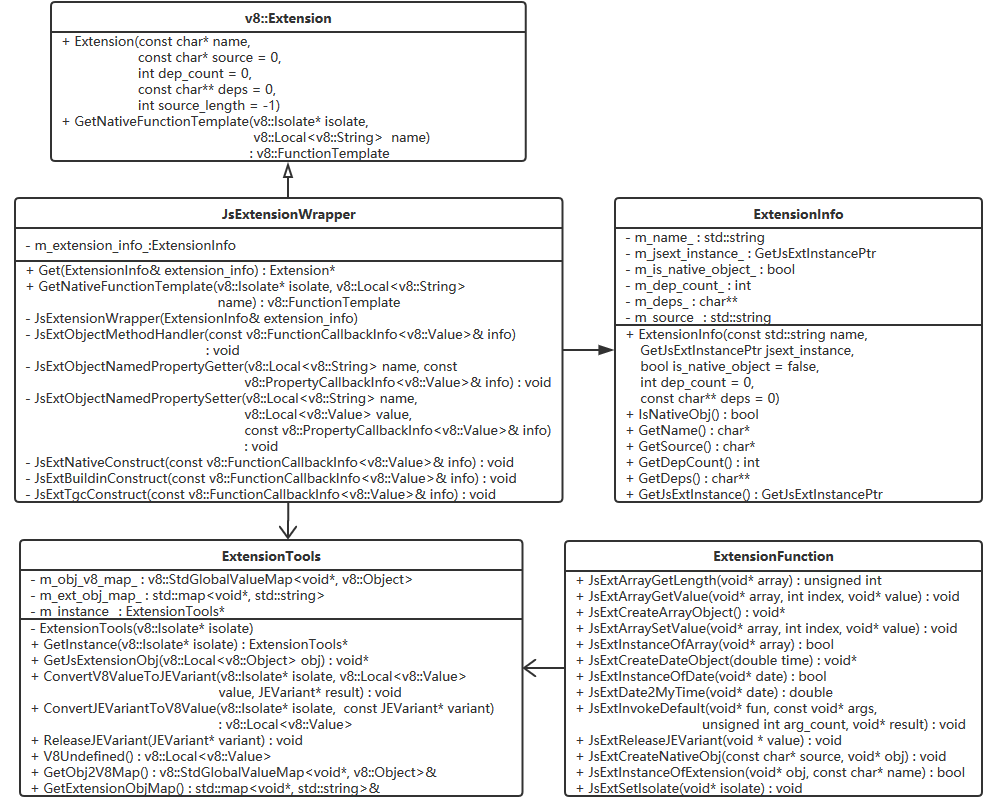
\includegraphics[width=\textwidth]{image/extension_framework/extension_framework_class.png} 
  \caption{extension framwork静态类图} \label{fig:extension_framework_class} 
\end{figure}

如第图~\ref{fig:extension_framework_class}所示:
v8扩展机制主要是继承v8内置的Extension类,通过重写其GetNativeFunctionTemplate方法来获取FunctionTemplate对象;
JsExtensionWrapper类主要就是封装创建出来的FunctionTemplate对象的一些特性,比如构造函数,属性拦截器,方法执行;
ExtensionInfo类主要记录了创建v8扩展所有需要的关键信息;ExtensionTools类主要是提供简易的函数,比如通过v8::Object类获取ExtensionBase对象,
将v8变量转换为扩展变量,将扩展变量转换为v8变量,释放扩展变量等;ExtensionFunction主要提供常用对外接口给js扩展调用。

\begin{figure}[H] 
  \centering 
  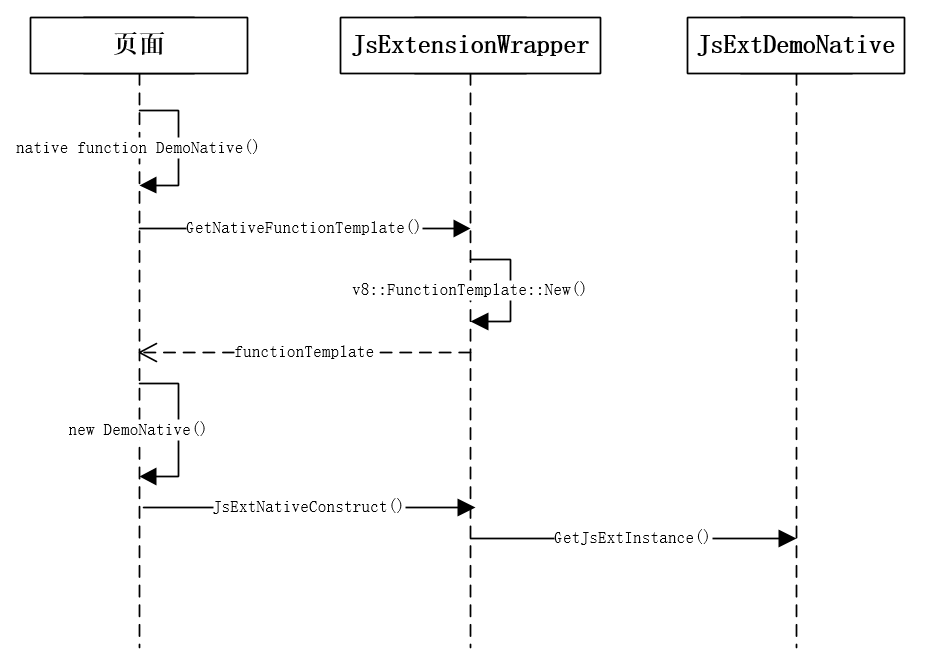
\includegraphics[width=\textwidth]{image/extension_framework/extension_construct_sequence.png} 
  \caption{js扩展对象创建时序图} \label{fig:extension_construct_sequence} 
\end{figure}

js扩展对象创建时序图如图~\ref{fig:extension_construct_sequence}所示:
\begin{itemize}
  \item 在页面加载时,v8::extension会注入页面代码native function DemoNative(),此时v8就会去创建DemoNative对应functionTemplate模板类。
  \item 当web开发人员在页面使用new DemoNative()时,functionTemplate模板类就会返回一个v8::Object实例对象给页面。
  \item 同理,针对内置对象,v8::extension会注入页面代码native function DemoBuildin()和var DemoBuildin = DemoBuildin()两段代码,
  此时由于DemoBuildin变量覆盖了DemoBuildin方法名,所以只能通过DemoBuildin执行对应方法和函数,不能再被new。
\end{itemize}

\begin{figure}[H] 
  \centering 
  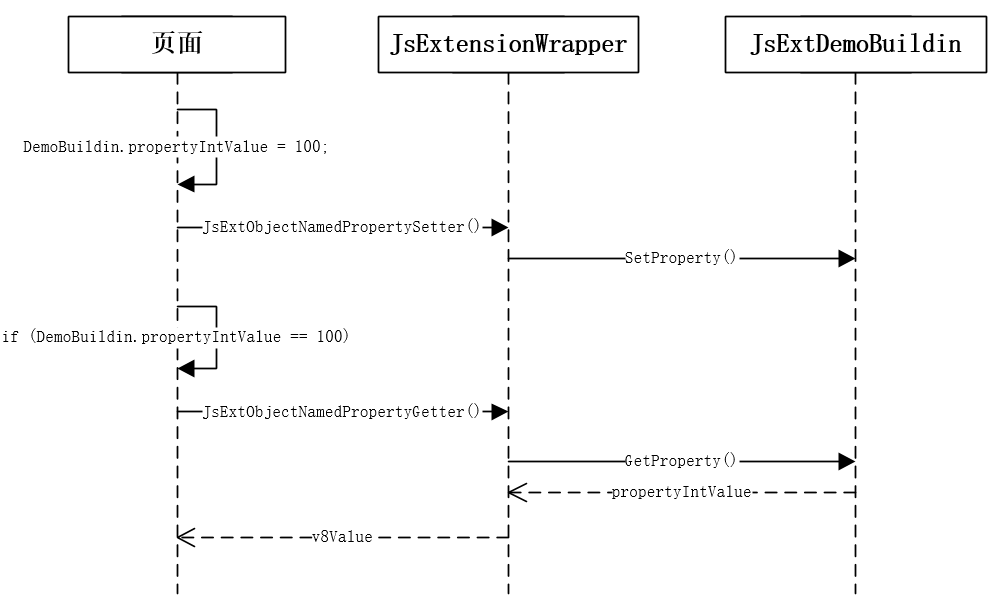
\includegraphics[width=\textwidth]{image/extension_framework/extension_property_sequence.png} 
  \caption{js扩展对象属性访问时序图} \label{fig:extension_property_sequence} 
\end{figure}

js扩展对象属性访问时序图如图~\ref{fig:extension_property_sequence}所示:
\begin{itemize}
  \item 由于在创建DemoBuildin对象时,对其ObjectTemplate模板类设置了拦截器特性,所以任何属性访问都会调用到拦截器的回调方法里。
\end{itemize}

\begin{figure}[H] 
  \centering 
  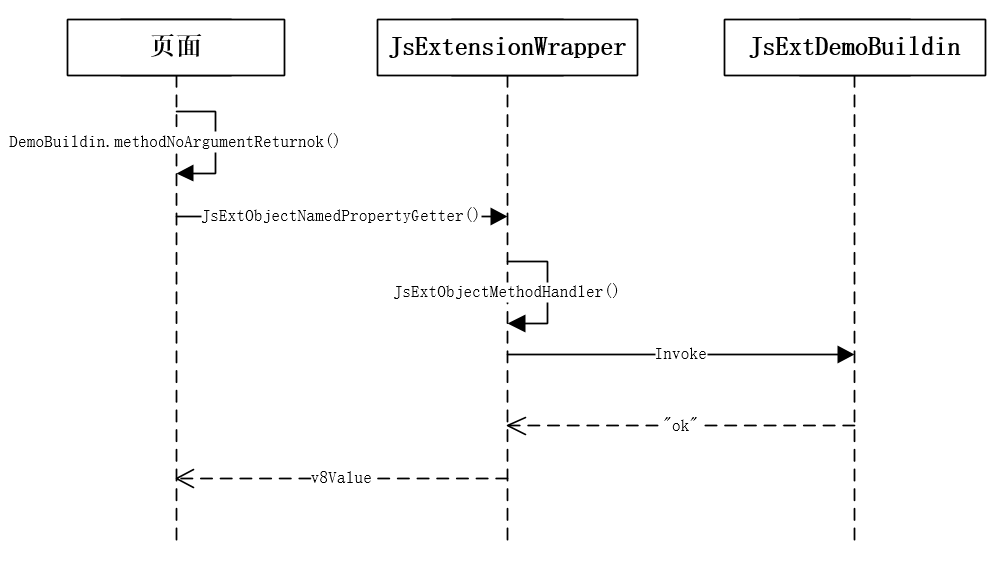
\includegraphics[width=\textwidth]{image/extension_framework/extension_function_sequence.png} 
  \caption{js扩展对象方法访问时序图} \label{fig:extension_function_sequence} 
\end{figure}

js扩展对象方法访问时序图如图~\ref{fig:extension_function_sequence}所示:
\begin{itemize}
  \item 同获取属性流程一致,当在拦截器回调函数里查询,如果属性没找到调用名,就去方法里找。
\end{itemize}

\section{Extension Framework垃圾回收机制}

对于内置对象,每次跳转页面,都会去调用其构造函数,此时回收机制的做法是先delete上个页面new出来的js扩展实例对象,再重新new一个js扩展实例对象,
然后绑定到v8 Object对象里。
\begin{spacing}{1.0}
\begin{lstlisting}[language={C++}]
void* delete_obj = ExtensionTools::GetJsExtensionObj(v8_obj);
  if (delete_obj) {
    ExtensionBase* ext_base = static_cast<ExtensionBase*>(delete_obj);
    delete ext_base;
    ext_base = NULL;
  }

  void* new_obj = NULL;
  extension_info->GetJsExtInstance()(NULL, 0, &new_obj);
  v8_obj->SetInternalField(ExtensionTools::JsExtBaseInternalField, v8::External::New(isolate, new_obj));
\end{lstlisting}
\end{spacing}

对于本地对象,每次创建对象时,我们会通过一个std::map保存js扩展实例对象指针以及name,当跳转页面,都会去调用tgc内置对象其构造函数,
将这个map里js扩展实例对象指针全部delete掉。
\begin{spacing}{1.0}
\begin{lstlisting}[language={C++}]
//在构造函数中将js扩展实例对象指针以及name保存到一个map中
void JsExtensionWrapper::JsExtNativeConstruct(const FunctionCallbackInfo<v8::Value>& info) {
  ...
  ExtensionTools* extension_tools = ExtensionTools::GetInstance(isolate);
  extension_tools->GetExtensionObjMap().insert(std::pair<void*, std::string>(new_obj, extension_info->GetName()));
  ...
}

//在tgc内置对象构造函数中将map中的js扩展实例对象指针全部delete掉
void JsExtensionWrapper::JsExtTgcConstruct(const FunctionCallbackInfo<v8::Value>& info) {
  ...
  ExtensionTools* extension_tools = ExtensionTools::GetInstance(isolate);
  std::map<void*, std::string>::iterator it;
  for (it = extension_tools->GetExtensionObjMap().begin(); it != extension_tools->GetExtensionObjMap().end(); it++) {
    ExtensionBase* ext_base = static_cast<ExtensionBase*>(it->first);
    if (ext_base) {
      delete ext_base;
      ext_base = NULL;
    }
  }
  ...
}
\end{lstlisting}
\end{spacing}



%---------------------------------------------------------------------

\ifx\withtbrowser\undefined
\else
\input{contents/extension_framework.tex}
\fi

\fi

\fi

\fi
